\chapter{Experimental results}\label{ch:experiments}
%************************************************ 

In this chapter, we start by detailing in section \ref{sec:technologies} the choice of technologies in order to obtain experimental results. After that, these results will be discussed in order of application in sections \ref{sec:res_fs} (feature selection), \ref{sec:res_so} (structure optimization) and \ref{sec:res_lo} (learning optimization). By the end, we will have empirical evidence to point us in promising directions, which we will subsequently address when we talk about conclusions and future work.

\section{Software and hardware}\label{sec:technologies}

	\subsection{Software}

		The first decision to make is which programming language to use. \texttt{Python} is the choice for the following reasons:

		\begin{itemize}

			\item
			Previous experience with the language in web and machine learning applications.

			\item
			Popularity of the language, which is a good indicator of community support. According to the \textit{StackOverflow} 2018 Survey \footnote{\href{https://insights.stackoverflow.com/survey/2018/\#technology-programming-scripting-and-markup-languages}{\textit{StackOverflow} 2018 Survey: Most popular technologies}}, it is one of the most popular languages, and more so if we compare it with those commonly associated with machine learning in the last few years.

			\item
			Popularity of its machine learning and deep learning frameworks. Well-established frameworks include \texttt{Scikit-learn} \footnote{\href{https://github.com/scikit-learn/scikit-learn}{\texttt{Scikit-learn} GitHub repository}}, \\ \texttt{Caffe} \footnote{\href{https://github.com/BVLC/caffe}{\texttt{Caffe} GitHub repository}}, \texttt{TensorFlow} \footnote{\href{https://github.com/tensorflow/tensorflow}{\texttt{TensorFlow} GitHub repository}} and \texttt{Theano} \footnote{\href{https://github.com/Theano/Theano}{\texttt{Theano} GitHub repository}}. The last two of them also function as backends for the high-level neural networks API \texttt{Keras} \footnote{\href{https://github.com/keras-team/keras}{\texttt{Keras} GitHub repository}}. If we look at the number of stars in their \textit{GitHub} repositories, we can see that they are widely acknowledged by the community.

		\end{itemize}

\newpage

		The next step is choosing the tools to support our work. Since one of the goals of this project was to learn about optimization techniques, the genetic algorithm has been implemented from scratch, although there are alternatives like \texttt{DEAP} \footnote{\href{https://github.com/DEAP/deap}{\texttt{DEAP} GitHub repository}} if one wishes to avoid the additional development effort.

		Data operations become faster and easier with \texttt{Numpy} \footnote{\href{https://github.com/numpy/numpy}{\texttt{Numpy} GitHub repository}}. This will allow us to manage populations in genetic algorithms, as well as perform basic operations in a vectorized way whenever we need them. It is also fully compatible with the other libraries.

		Building machine learning models from scratch too is understandably out of the question. For this reason, we will rely on \texttt{Scikit-learn} for general machine learning algorithms and metrics, and on \texttt{Keras}---with its default \texttt{TensorFlow} backend---for neural networks.

		Lastly, many charts will be generated using \texttt{R} \footnote{\href{https://www.r-project.org/}{\texttt{R} Project website}}, which provides simple and powerful functionality for this task.

	\subsection{Hardware}

		We can make a distinction in this regard between the main development system, used for testing and debugging, and the dedicated servers for full-scale experimentation:

		\begin{itemize}

			\item
			Development system:

			\begin{itemize}

				\item
				Intel® Core™ i5-3470 CPU @ 3.20GHz, 8GB DDR3.
				\item
				NVIDIA GeForce® GTX 960, 2GB GDDR5.

			\end{itemize}

			\item
			First dedicated server:

			\begin{itemize}

				\item
				Intel® Xeon® E5-2620 v2 @ 2.10GHz, 32GB DDR3.
				\item
				NVIDIA Tesla® K20c, 5GB GDDR5.

			\end{itemize}

			\item
			Second dedicated server:

			\begin{itemize}

				\item
				Intel® Xeon® E5-2620 v4 @ 2.10GHz, 32GB DDR4.
				\item
				NVIDIA Tesla® K40m, 12GB GDDR5.

			\end{itemize}

			\item
			Third dedicated server:

			\begin{itemize}

				\item
				Two Intel® Xeon® E5-2620 v4 @ 2.10GHz, 32GB DDR4.
				\item
				NVIDIA Tesla® K40m, 12GB GDDR5.

			\end{itemize}

		\end{itemize}

\newpage

\section{Feature selection}\label{sec:res_fs}

	Determining the right configuration for the genetic algorithm---or rather, even one that is good enough---is no trivial task. Early experimentation seemed to point to a high crossover probability, but especially to a high mutation probability (ultimately set to 1). We will elaborate on that soon.

	Let us start by comparing three different crossover operators: \textit{Uniform}, \textit{Single-point} and \textit{Two-point}. We will work with a population of 300 individuals and 150 generations. We will set a 0.9 crossover probability after which a mutation will always ensue. A maximum of 50 active features will be allowed in each individual. The fitness criteria will take into account the Kappa value (for test accuracy) and a 5-fold cross-validation (for generalization assessment) measured for Logistic Regression.

	We will do an initial test run on each subject (104, 107 and 110). 

	Figure \ref{gfx:fs_crossover_kappa} displays the evolution of the mean Kappa error for all crossover operators in all three subjects.

    \begin{figure}[h]

        \begin{center}

        	\setlength{\fboxrule}{0pt}
            \fbox{
				\begin{varwidth}{\textwidth}
					\centering
					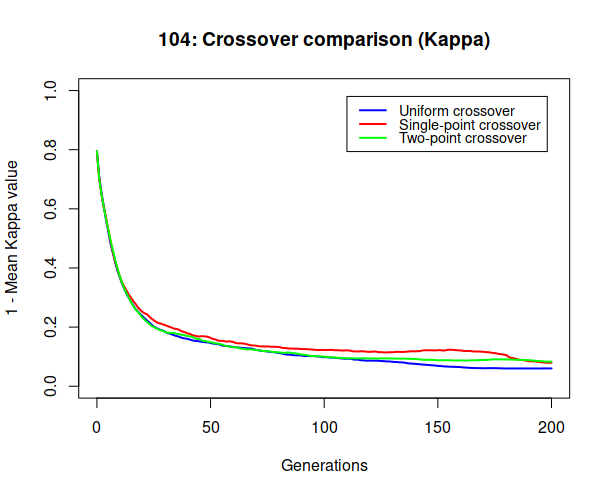
\includegraphics[width=0.45\textwidth]{gfx/FS_Crossover_Kappa_104.png}
				\end{varwidth}
			}
			\fbox{
				\begin{varwidth}{\textwidth}
					\centering
					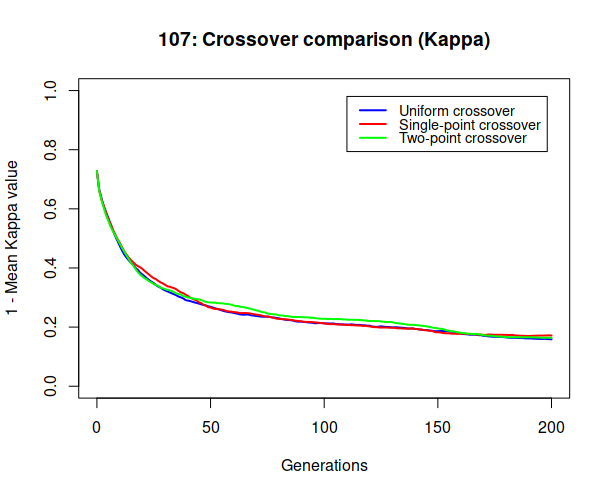
\includegraphics[width=0.45\textwidth]{gfx/FS_Crossover_Kappa_107.png}
				\end{varwidth}
			}
            \fbox{
				\begin{varwidth}{\textwidth}
					\centering
					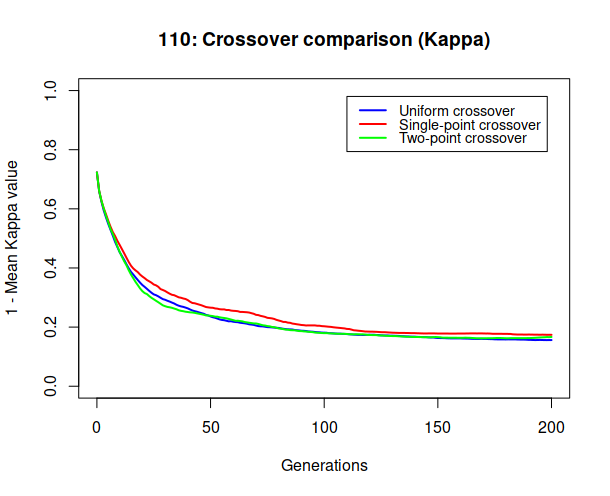
\includegraphics[width=0.45\textwidth]{gfx/FS_Crossover_Kappa_110.png}
				\end{varwidth}
			}

		\end{center}
		\caption[Kappa loss comparison for different crossovers]{Comparison of Kappa loss evolution over time with different crossover operators.}\label{gfx:fs_crossover_kappa}

	\end{figure}

	We can identify appreciable differences between the three curves: the blue one (uniform crossover) shows consistently better results than the other two, and the red one (single-point crossover) appears to be the worst.

\newpage

	Let us move on now to the same type of chart but with the cross-validation error (Figure \ref{gfx:fs_crossover_cv}). Again, the uniform crossover operator achieves the top performance across all individuals and the single-point crossover operator often lags behind.

	\begin{figure}[h]

        \begin{center}

        	\setlength{\fboxrule}{0pt}
            \fbox{
				\begin{varwidth}{\textwidth}
					\centering
					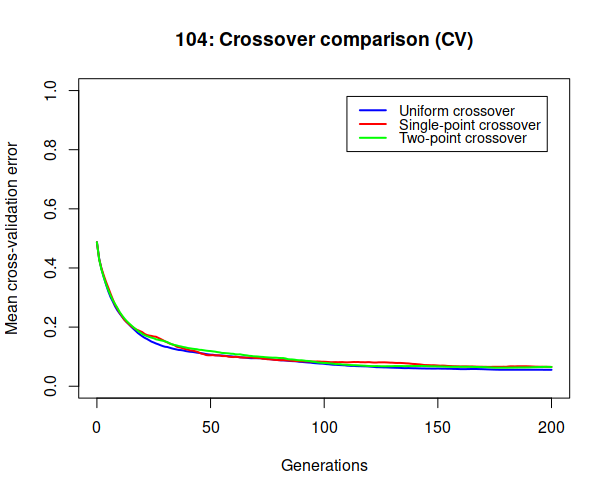
\includegraphics[width=0.45\textwidth]{gfx/FS_Crossover_CV_104.png}
				\end{varwidth}
			}
			\fbox{
				\begin{varwidth}{\textwidth}
					\centering
					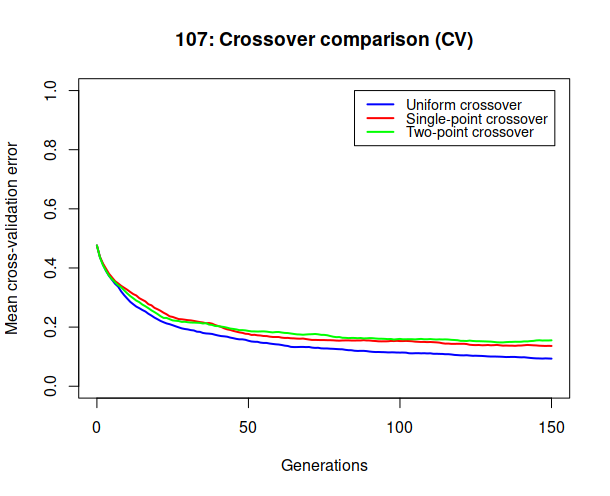
\includegraphics[width=0.45\textwidth]{gfx/FS_Crossover_CV_107.png}
				\end{varwidth}
			}
            \fbox{
				\begin{varwidth}{\textwidth}
					\centering
					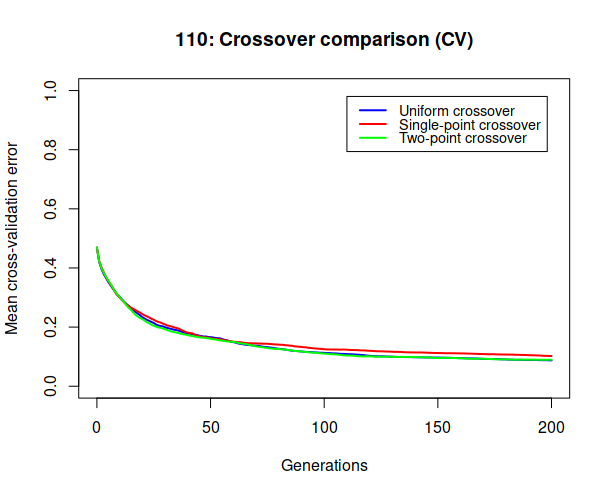
\includegraphics[width=0.45\textwidth]{gfx/FS_Crossover_CV_110.png}
				\end{varwidth}
			}

		\end{center}
		\caption[CV loss comparison for different crossovers]{Comparison of cross-validation loss evolution over time with different crossover operators.}\label{gfx:fs_crossover_cv}

	\end{figure}

	We seem to be spotting a trend that depends on the crossover operator. However, is it wise to extrapolate from only one test run? The answer is no: the running times allow us to repeat the experiment several times and find out whether their differences are statistically significant.

	As a compromise between quantity of samples and time expended, we will analyze 15 samples per crossover operator using their Kappa values. Table \ref{table:crossover_kappa} shows the resulting values for all possible combinations:

	\vspace{0.3cm}

	\begin{table}[h]

        \centering
        \setlength\arrayrulewidth{0.8pt}

        \begin{tabular}{| >{\centering\arraybackslash}m{0.5in} | >{\centering\arraybackslash}m{1.1in} |  >{\centering\arraybackslash}m{1.1in} | >{\centering\arraybackslash}m{1.1in} |}

            \hline
            \rowcolor{RoyalBlue}
            \textbf{Subject} & \textbf{Uniform} & \textbf{Single-point} & \textbf{Two-point} \\
            \hline
            \textbf{104} & $0.06534 \pm 0.0074$ & $0.08619 \pm 0.0102$ & $0.07941 \pm 0.0119$ \\
            \hline
            \textbf{107} & $0.15202 \pm 0.0132$ & $0.18004 \pm 0.0137$ & $0.17725 \pm 0.0150$ \\
            \hline
            \textbf{110} & $0.14829 \pm 0.0138$ & $0.17131 \pm 0.0158$ & $0.16569 \pm 0.0187$ \\
            \hline

        \end{tabular}

        \caption{Comparison of average Kappa values for the three subjects and the three crossover operators.}\label{table:crossover_kappa}

    \end{table}

    The average performance of each operator seems to be what we expected. Additionally, the uniform crossover appears to produce slightly more stable results, judging from the standard deviation. Next, and not making assumptions about normality, we will perform a \textit{Kruskal-Wallis} test to see if their differences are worth considering. The \textit{p-values} are displayed in Tables \ref{table:crossover_kruskal_104}, \ref{table:crossover_kruskal_107} and \ref{table:crossover_kruskal_110}, with values below $0.05$ representing meaningful differences ($95\%$ confidence interval).

    \vspace{0.0cm}

	\begin{table}[h]

        \centering
        \setlength\arrayrulewidth{0.8pt}

        \begin{tabular}{| >{\centering\arraybackslash}m{0.9in} |  >{\centering\arraybackslash}m{0.9in} | >{\centering\arraybackslash}m{0.9in} |}

            \hline
            \rowcolor{RoyalBlue}
            \textbf{104} & \textbf{Single-point} & \textbf{Two-point} \\
            \hline
            \cellcolor{RoyalBlue}\textbf{Uniform} & $p = 0.000027$ & $p = 0.000835$ \\
            \hline
            \cellcolor{RoyalBlue}\textbf{Single-point} & \cellcolor{lightgray} & \textcolor{red}{$p = 0.056282$} \\
            \hline

        \end{tabular}

        \caption{Comparison of p-values for the crossover operators (subject 104).}\label{table:crossover_kruskal_104}

    \end{table}

    \begin{table}[h]

        \centering
        \setlength\arrayrulewidth{0.8pt}

        \begin{tabular}{| >{\centering\arraybackslash}m{0.9in} |  >{\centering\arraybackslash}m{0.9in} | >{\centering\arraybackslash}m{0.9in} |}

            \hline
            \rowcolor{RoyalBlue}
            \textbf{107} & \textbf{Single-point} & \textbf{Two-point} \\
            \hline
            \cellcolor{RoyalBlue}\textbf{Uniform} & $p = 0.000023$ & $p = 0.000104$ \\
            \hline
            \cellcolor{RoyalBlue}\textbf{Single-point} & \cellcolor{lightgray} & \textcolor{red}{$p = 0.678133$} \\
            \hline

        \end{tabular}

        \caption{Comparison of p-values for the crossover operators (subject 107).}\label{table:crossover_kruskal_107}

    \end{table}

    \begin{table}[h]

        \centering
        \setlength\arrayrulewidth{0.8pt}

        \begin{tabular}{| >{\centering\arraybackslash}m{0.9in} |  >{\centering\arraybackslash}m{0.9in} | >{\centering\arraybackslash}m{0.9in} |}

            \hline
            \rowcolor{RoyalBlue}
            \textbf{110} & \textbf{Single-point} & \textbf{Two-point} \\
            \hline
            \cellcolor{RoyalBlue}\textbf{Uniform} & $p = 0.000454$ & $p = 0.006561$ \\
            \hline
            \cellcolor{RoyalBlue}\textbf{Single-point} & \cellcolor{lightgray} & \textcolor{red}{$p = 0.299489$} \\
            \hline

        \end{tabular}

        \caption{Comparison of p-values for the crossover operators (subject 110).}\label{table:crossover_kruskal_110}

    \end{table}

    As we can see, the single-point and two-point crossovers show no statistically significant differences in their recorded results.

    The computational impact of either operator is negligible against the much more intensive fitness evaluations, so there is no reason not to consider the uniform crossover as our pick from now on. The last thing to do before moving on is attempt to explain why this happens. 

    On one hand, $n$-point crossovers merge large blocks from both parents; this leads to a not-so-optimal information transfer when trying to pick a handful of features from a pool of 3600.

    On the other hand, the uniform crossover is often said to be very disruptive, due to randomly choosing elements for which the parents do not agree. However, when only a small portion $k$ of features is active at a time, the disruption is at most $2k$ elements (the rest are inactive features); on top of that, features in which both parents agree are always kept. This makes the uniform crossover excel at \textit{exploitation} while also helping in \textit{exploration}. Together with frequent mutations, this is probably the key of the performance gain of the algorithm.

%\section{Structure optimization}\label{sec:res_so}

%\section{Learning optimization}\label{sec:res_lo}